\section{Objektorientierung}

Objektorientierung soll es erleichtern, eine Abbildung der Realität zu erstellen. 
Viele Dinge aus der Wirklichkeit können als Modell dargestellt / simplifiziert werden. 
Diese Modelle können in Software in sogenannte Objekte \texttt{umgewandelt} werden.

\subsection{Objekte}

Objekte stellen Dinge, Sachverhalte oder Prozesse dar. Sie sind ein rein gedankliches Konzept.\\
Sie kennzeichnen sich durch:

\begin{itemize}[itemsep=1pt, parsep=0pt]
    \item eine \textbf{Identität}, welche es erlaubt Objekte voneinander zu unterscheiden
    \item \textbf{statische Eigenschaften} zur Darstellung des \textbf{Zustandes} des Objekts in Form von \textbf{Attributen}
    \item \textbf{dynamische Eigenschaften} zur Darstellung des \textbf{Verhaltens} des Objekts in Form von \textbf{Methoden}
\end{itemize}


\subsection{Klassen \& Instanzen}

Ähnliche Objekte können in \textbf{Klassen} zusammengefasst werden, um Programmieraufwand tiefer zu halten. 
Verwendete Objekte werden als \textbf{Instanz} eingesetzt. Diese Objekte haben dieselben Attribute, allerdings andere Werte.\\
Eine Beispielklasse:

\lstinputlisting{code/03_Objektorientierung/class_example.cpp}\vspace{-1em}

\subsubsection{Reihenfolge der Header-Datei (.h)}

\begin{enumerate}[itemsep=1pt, parsep=0pt]
    \item Dateikommentar mit Lizenzvereinbarung.
    \item \textit{\color{blue} \texttt{Includes} des verwendete System Header \texttt{<\dots>}}
    \item \textit{\color{blue} \texttt{Includes} der Projektbezogenen Header \texttt{"\dots"}}
    \item \textit{\color{blue} Definition von Konstanten}
    \item \textit{\color{blue} Typedef's und Definitionen von Strukturen}
    \item \textit{\color{blue} allenfalls extern-Deklaration von Global-Variablen}
    \item \textit{\color{blue} Funktionsprototypen, ink. Kommentar der Schnittstelle, bzw. Klassendeklarationen}
\end{enumerate}

\begin{itemize}
    \item Die \textit{blauen} Punkte müssen sich im Includeguard befinden(\#pragma once). 
    \item Pro Header-Datei sollte nur eine Oberklasse deklariert sein. 
    \item Kleine Unterklassen können im gleichen Header stehen.
    \item Kein \lstinline[language=C++]|using namespace ...| in header files
\end{itemize}

\subsubsection{Reihenfolge der Implementation (.cpp)}

\begin{enumerate}[itemsep=1pt, parsep=0pt]
    \item Dateikommentar mit Lizenzvereinbarung
    \item \texttt{includes} der eigenen Header
    \item \texttt{includes} der Projektbezogenen Header
    \item \texttt{includes} der verwendeten System Header
    \item allenfalls globale und statische Variablen
    \item Präprozessor-Direktiven
    \item Funktionsprototypen von lokalen, internen Funktionen (in nameless Namespace)
    \item Definition von Funktionen und Klassen (\crd{Kommentare nicht wiederholen})
\end{enumerate}

\subsection{UML}

Die \texttt{Unified Modeling Language} ist eine normierte Sprache um Objekte grafisch 
darzustellen, \textbf{programmierspracheunabhängig}.

\subsubsection{UML-Klassendiagramm Notation}

Besteht immer aus 3 Boxen:\vspace{1em}

\noindent
\begin{minipage}{0.4\columnwidth}
\begin{center}
        \begin{tikzpicture}
        \node [umlclass] (Student) { % see preamble umclass style
            \centering \textbf{Student}
            \nodepart{second}
                + IDNumber : int \\
                \# name : string \\
                - bierkonsum : float \\
                \# investedTimeInET : int
            \nodepart{third}
                - doStuff(time : int) \\
                + \textit{useless()}
        };
    \end{tikzpicture}
\end{center}
\end{minipage}
\begin{minipage}{0.57\columnwidth}
    \begin{itemize}
        \raggedright
        \item Zu oberst der Name 
        \item In der Mitte Attribute(Variablen)
        \item Unten Methoden.
        \item Methoden und Attribute fangen mit einem Symbol an, welches die \textbf{Sichtbarkeit} 
                definiert und haben ein bestimmtes Merkmal:
        \item Parole come \lstinline[language=C++]|void| o \lstinline[language=C++]|const| sono specifiche per linguaggio, da non includere
    \end{itemize}
\end{minipage}\vspace{1em}

\begin{itemize}[itemsep=1pt, parsep=0pt]
    \item + : public (überall sichtbar)
    \item - : private (nur in  aktueller Klasse sichtbar)
    \item \# : protected (in aktueller und Unterklassen sichtbar)
    \item \textit{Italic} : Funktion oder Klasse ist Abstrakt (=0)
    \item \underline{Unterstrichen} : Funktion oder Attribut ist static
    \item \verb|<Name der Klasse>| :  Konstruktor (ohne \verb|<>|)
    \item $\sim$\verb|<Name der Klasse>| : Destruktor (ohne \verb|<>|)
\end{itemize}



\subsection{class vs struct}

Eine class und struct können fast identisch verwendet werden. 
Eine class hat \textbf{standardmässig Sichtbarkeit private} sonst muss explizit mit \lstinline[language=C++]|public:| gekennzeichnet, Struct public(wenn nichts definiert wird).

\subsubsection{Zugriffsschutz}
\begin{tabular}{|l|l|}
    \hline
    \textbf{Modificatore} & \textbf{Descrizione e Best Practice} \\ \hline
    \lstinline[language=C++]|public| & Accessibili dall'interno e dall'esterno della classe. \\ 
    & $\rightarrow$ Quasi tutti i \textbf{metodi} sono pubblici. \\ 
    & $\rightarrow$ \textbf{attributi} non dovrebbero \textit{mai} essere pubblici. \\ \hline
    \lstinline[language=C++]|protected| & Accessibili dall'interno della classe e dalle \textbf{classi derivate}. \\ 
    & $\rightarrow$ Da utilizzare con parsimonia. \\ \hline
    \lstinline[language=C++]|private| & Accessibili \textbf{solo} all'interno della classe stessa. \\ 
    & $\rightarrow$ Per tutti gli attributi e per metodi locali specifici. \\ \hline
\end{tabular}

\subsection{Inkludierte Dokumentation}

Mann kann im H-File direkt die Dokumentation zu der Schnittstelle schreiben. 
Das ermöglicht das einfachere Verwenden der Schnittstelle.

\lstinputlisting{code/03_Objektorientierung/codedocumentation.cpp}

Es kann immer mehr geschrieben werden, man sollte sich aber auf das Nötige beschränken.

\section{Konstruktoren und Destruktoren}

I costruttori (CTOR) e i distruttori (DTOR) sono metodi speciali che gestiscono il ciclo di vita di un oggetto. Entrambi hanno lo stesso nome della classe e \textbf{non} hanno alcun tipo di ritorno (nemmeno \lstinline[language=C++]|void|).

\subsection{Konstruktoren (CTOR)}

Il compito principale del CTOR è l'inizializzazione "pulita" di tutti gli attributi della classe.

\begin{itemize}
    \item \textbf{Default-Konstruktor:} Non ha parametri. Viene invocato automaticamente se l'oggetto è dichiarato senza argomenti (es. \lstinline[language=C++]|Stack s;|). Se non definito, il compilatore ne crea uno implícito (che però non inizializza i tipi primitivi).
    \item \textbf{Copy-Konstruktor:} Riceve una \lstinline[language=C++]|const|-Referenz alla propria classe (\lstinline[language=C++]|TString(const TString& s)|). Viene usato per creare un oggetto come copia di uno esistente.
    \item \textbf{Explicit-Konstruktor:} Marcando un CTOR a parametro singolo con \lstinline[language=C++]|explicit|, si impediscono conversioni implicite indesiderate (es. \lstinline[language=C++]|TString s = 5;|).
\end{itemize}

Werden verschiedene Konstruktoren definiert, muss der Default zuerst aufgerufen werden, wenn dieser erhalten bleiben soll.

\subsubsection{Best Practices di Inizializzazione}
Una delle responsabilità primarie del costruttore è garantire che l'oggetto nasca in uno stato valido. Ciò implica che \textbf{tutti} gli attributi della classe debbano essere inizializzati su un valore definito.

\begin{itemize}
    \item \textbf{Assegnamento nel corpo (\ref{chap:ctor_dtor_example}):} Meno efficiente, i membri vengono prima creati con valori predefiniti e poi sovrascritti.
    \item \textbf{Initialisierungsliste (\ref{chap:user_ctor}):} Il metodo preferito per motivi di efficienza; gli attributi vengono inizializzati direttamente al momento della creazione.
    \item \textbf{Member In-Class Initialization:} (Da C++11) Permette di impostare valori di default direttamente nella dichiarazione della classe, semplificando i costruttori ed evitando dimenticanze.
\end{itemize}

\subsection{Gestione Memoria: Shallow vs. Deep Copy}

Quando una classe gestisce puntatori a memoria allocata sul Heap (\lstinline[language=C++]|new|), il comportamento di default è critico:

\begin{description}
    \item[Shallow Copy (Default):] Il compilatore copia solo l'indirizzo del puntatore. Entrambi gli oggetti puntano alla stessa memoria. Se uno la libera, l'altro punta a memoria non valida (\textit{Double Free} o \textit{Segmentation Fault}).
    \item[Deep Copy (Manuale):] \textbf{\color{red}È necessario} definire un Copy-Konstruktor proprio che allochi nuovo spazio sul Heap e copi i dati effettivi.
\end{description}

\subsection{Destruktor}

Ein Destruktor eintfernt eine Instanz aus dem Speicher, 
hat keine Aufrufparameter und auch kein Rückgabewert. 
Es kann immer nur \textbf{einen} Destruktor geben. 
Wenn der Destruktor fertig ist, sollte kein Speicher mehr vom Objekt belegt sein.\\
Destruktoren sollten immer \textbf{virtuell definiert werden} (siehe \ref{Virtual}). 
Mit anderen virtuellen Funktionen \textbf{müssen} sie virtuel definiert werden. 
Der Funktionsname beginnt mit einer Tilde($\sim$). 
Der Destruktor wird evtl. auch Implizit aufgerufen z.b., wenn aus einer Funktion wieder herausgesprungen wird. 

\subsection{Beispiel}\label{chap:ctor_dtor_example}

\lstinputlisting{code/03_Objektorientierung/constructor.cpp}

\section{Initialisierungslisten und direkte Initialisierung}

Die Initialisierung von Datentypen kann auf verschiedene Arten erreicht werden. 
Es wird zwischen Zuweisung und Initialisierung unterschieden.

\subsection{POD's}

\texttt{plain old datastructure} / built in datatypes

\lstinputlisting{code/03_Objektorientierung/pod_init.cpp}

\subsection{Non PODs}

\lstinputlisting{code/03_Objektorientierung/non_pod_init.cpp}

\subsection{User defined Constructor}\label{chap:user_ctor}

Um eine Klasse richtig initialisieren zu können muss der Ctor korrekt definiert werden. 
Eine sogenannte \textbf{Initialisierungsliste} wird verwendet:

\lstinputlisting{code/03_Objektorientierung/userdefined_ctro.cpp}

\section{Assertions}
Assertions sollten Annahmen über korrekte Wertebelegung darstellen. 

Sie sind kein C spezifisches Konzept und sollten \textbf{nur zu Testzwecken} eingesetzt werden. 
Im Releasebuild sollten sie deaktiviert werden. 
Dafür gibt es spezifische Präprozessorflags.
Der Header \textbf{$<$assert.h$>$} bzw. \textbf{$<$cassert$>$} stellt hierfür ein Präprozessor-Makro \lstinline[language=C++]|assert(Bedingung)| zur Verfügung, um solche Zusicherungen auszudrücken.\\
\textbf{Beispiel}:

\lstinputlisting{code/03_Objektorientierung/assertions.cpp}

Das obige Beispiel hat eine Assertion. 
Diese würde im Test, falls ein Nullpointer übergeben wird ein Fehler ausgegeben.

\section{This-Pointer}

Mit dem \texttt{this Pointer} kann ein Pointer des aufrufenden Objekt zurückgegeben werden. Bsp:

\lstinputlisting{code/03_Objektorientierung/this_pointer.cpp}

Nacheinander werden diese Funktionen durchlaufen da Funktion(2) vom zurückgegebenen Pointer aus Funktionsaufruf 1 aus gerufen wird.
Die funktion wird \textbf{Kaskadiert}


\section{Overloading}

Operator Overloading bedeutet das bestehende Operatoren \texttt{überladen} werden im Sinne neu definiert / darüber geladen. 
Sie erhalten \textbf{neue Bedeutung} für eine Klasse.


\subsection{Methodenoverloading}
\begin{itemize}
    \item \textbf{Definizione}: Stesso nome per funzioni con parametri diversi (tipo, numero o ordine).
    \item \textbf{Firma}: Composta da \textit{Nome + Parametri}. Il tipo di ritorno è \textbf{escluso}.
    \item \textbf{Regola}: Se differiscono solo per il tipo di ritorno, il compilatore genera un errore.
    \item \textbf{Best Practice}: Usare l'overloading solo per operazioni comparabili e \textbf{non mescolarlo mai con i parametri di default.}
\end{itemize}

\begin{center}
    
    \begin{tabular}{lll}
        \toprule
        \textbf{Caratteristica} & \textbf{Overloading} & \textbf{Parametri Default} \\
        \midrule
        Memoria & Più funzioni & Singola funzione \\
        Manutenzione & Maggiore & Minore \\
        Flessibilità & Tipi diversi & Valori predefiniti \\
        \bottomrule
    \end{tabular}
\end{center}

\lstinputlisting[language=c++]{code/03_Objektorientierung/method_overloading.cpp}

\subsection{Operator overloading}

Es können die inkludierten Operatoren von C++ überladen werden. 
% \begin{itemize}
%     \item Die Anzahl an Operanden und die Bindungsrichtung (links nach rechts) kann \textbf{nicht} verändert werden.
%     \item Die Präzedenz (Vorrangregeln) kann \textbf{nicht} verändert werden.
%     \item Es können \textbf{keine} neuen Operatoren erfunden werden.
% \end{itemize}

Erlaubte Operatoren sind:\\
\begin{tabular}{lllllllll}
    +            & -               & *           & ⁄                      & \%                           & $\wedge$                & \&                            & $|$              & $\sim$          \\
    !            & =               & \textless{} & \textgreater{}         & +=                           & -=                      & *=                            & ⁄=               & \%=             \\
    $\wedge$=    & \&=             & $|$=        & \textless{}\textless{} & \textgreater{}\textgreater{} & \textless{}\textless{}= & \textgreater{}\textgreater{}= & ==               & !=              \\
    \textless{}= & \textgreater{}= & \&\&        & $\|$                   & ++                           & $--$                    & ,                             & -\textgreater{}* & -\textgreater{} \\
    ( )          & {[} {]}         & new         & delete                 & new{[} {]}                   & delete{[} {]}           &                               &                  &                
\end{tabular}\medskip

Nicht erlaubte Operatoren sind: '\lstinline[language=C++]|.| \quad \lstinline[language=C++]|.*| \quad \lstinline[language=C++]|::| \quad \lstinline[language=C++]|?:| \quad \lstinline[language=C++]|sizeof| \quad \lstinline[language=C++]|typeid|'.

Es wird zwischen Overloading als \textit{globalen Funktion} und als \textit{Klassen-Methode} unterschieden.

\subsubsection{Als Methode (Member function)}

Ein Operator kann als Methode einer Klasse definiert werden. Dies ist der Standardfall, wenn der \textbf{linke Operand} ein Objekt der eigenen Klasse ist.

Der linke Operand (Objekt selbst) ist dabei implizit, weshalb die Methode \textbf{einen Parameter weniger} annimmt als die globale Variante.\\
Syntax: \lstinline[language=C++]|<returntype> operator<typ>(type in);|

\begin{itemize}
    \item \textbf{Visibilità a livello di Classe:} In C++, il controllo degli accessi (\lstinline[language=C++]|private|) agisce a livello di \textbf{classe}, non di singolo oggetto.
    \item \textbf{Accesso Incrociato:} \cor{Un metodo della classe $A$ ha il permesso di accedere ai membri privati di \textit{qualsiasi} istanza di tipo $A$.}
    \item \textbf{Applicazioni:} Questa caratteristica è indispensabile per implementare correttamente l'overloading degli operatori (es. \lstinline[language=C++]|operator+|), i costruttori di copia e i metodi di confronto, dove un oggetto deve leggere i dati interni di un suo 'simile'.
\end{itemize}

\lstinputlisting{code/03_Objektorientierung/operator_overloading_method.cpp}

\textbf{Zwingend als Elementfunktion zu implementieren}
\begin{itemize}
    \item Zuweisung (\lstinline[language=C++]|=|, \lstinline[language=C++]|+=|, etc.)
    \item Index \lstinline[language=C++]|[]|
    \item Funktionsaufruf \lstinline[language=C++]|()|
    \item Zeigeroperator \lstinline[language=C++]|->|
\end{itemize}

\subsubsection{Als globale Funktion (Global)}

Globales Overloading wird \textbf{zwingend benötigt}, wenn der \cor{\textbf{linke Operand} \textit{nicht} 
von der eigenen Klasse ist.} Typische Beispiele sind:
\begin{itemize}
    \item Ein primitiver Datentyp links (z.B. \verb|string + TString|).
    \item I/O Stream-Operatoren wie \textless{}\textless{}, bei denen der linke Operand ein Stream-Objekt ist (z.B. \verb|std::cout << obj|).
\end{itemize}

Syntax: \verb|<returntype> operator<type>(type val1, type val2);|\medskip

\textbf{Friend Keyword:}\\
Oft müssen globale Operatorfunktionen auf private Daten der Klasse zugreifen. In diesem 
Fall werden sie innerhalb der Klasse mit dem Keyword \lstinline[language=C++]|friend| deklariert. 
Dadurch erhalten sie als globale Funktionen Zugriff auf \textbf{alle privaten Attribute 
und Methoden} der Klasse, ohne selbst Teil der Klasse (Methode) zu sein. 

\crd{\textit{Achtung}: Friend-Funktionen sollten gezielt eingesetzt werden.}

\lstinputlisting{code/03_Objektorientierung/operator_overloading_global.cpp}

\textbf{Beispiel I/O Streams (\lstinline[language=C++]|<<|):}\\
Damit Verkettungen wie \verb|cout << a << b;| funktionieren, muss als Rückgabewert eine Referenz auf den \verb|ostream| geliefert werden (\verb|return os;|).
\lstinputlisting[language=C++]{code/03_Objektorientierung/03_Objektorientierung_snippet_1.cpp}

\subsubsection{Operatoren und Typumwandlungen}
\begin{itemize}
    \item Per evitare di dover definire innumerevoli varianti di un operatore per ogni combinazione di tipi, è possibile sfruttare le \textbf{conversioni di tipo definite dall'utente}.
    \item Singolo operatore può gestire diversi input se esiste un costruttore in grado di convertire tali tipi nella classe di destinazione.
\end{itemize}

\lstinputlisting[language=C++]{code/03_Objektorientierung/operatoren_typumwandlung.cpp}

\section{Getter \& Settermethoden}

Getter und Settermethoden werden Typischerweise verwendet um Lese und Schreibzugriffe auf eine Klasse zu regeln.

Attribute sind \textbf{alle Parameter einer Klasse}.
Mit einer Get oder Set Methode kann der Zugriff auf diese kontrolliert / angepasst werden.\medskip

\cor{\lstinline[language=C++]|const| after the funtion name declares that the method cannot modify any Attribute} 

\myul{immer fur Selector (Getter) benutzen}

\lstinputlisting{code/03_Objektorientierung/getter_settermethoden.cpp}

\subsubsection{Mutable}
Si può permettere a determinati attributi di essere 
modificati da metodi \lstinline[language=C++]|const| con la keyword \lstinline[language=C++]|mutable|,
\textbf{usare il meno possibile}
\begin{lstlisting}
...
mutable int error;
...
\end{lstlisting}

\subsubsection{Const correctness}
\begin{itemize}
    \item \textbf{Sola Lettura:} Un oggetto dichiarato come \lstinline[language=C++]|const| può invocare \textit{solo} metodi dichiarati \lstinline[language=C++]|const|.
    \item \textbf{Sicurezza:} Se un metodo non è marcato \lstinline[language=C++]|const|, il compilatore assume che possa modificare l'oggetto e ne impedisce l'uso su istanze costanti per evitare effetti collaterali indesiderati.
\end{itemize}

\example{}
\lstinputlisting[language=C++]{code/03_Objektorientierung/03_Objektorientierung_snippet_2.cpp}

\section{Vererbung}

Vererbung erlaubt es Attribute und Methoden von anderen Klassen zu übernehmen. 
Die Oberklasse, Baisklasse oder Superklasse \texttt{vererbt} an eine Unterklasse, derived class oder eine Spezialisierung. 
Bei der Vererbung werden immer \textbf{alle} Attribute oder Methoden weitergegeben. 

\subsubsection{UML}

In einem UML Diagramm wird vererbung wie folgt dargestellt:\\
\noindent
\begin{minipage}{0.6\columnwidth}
        \begin{tikzpicture}[>=Triangle]
        % Nodo Superclasse
        \node[umlclass] (super) {
            \hfil \textbf{Superklasse} \hfil
            \nodepart{second}
            Attribute
            \nodepart{third}
            Methoden
        };

        % Nodo Unterklasse posizionato a destra
        \node[umlclass, right=1cm of super] (unter) {
            \hfil \textbf{Unterklasse} \hfil
            \nodepart{second}
            Attribute
            \nodepart{third}
            Methoden
        };

        % Freccia di ereditarietà (Generalizzazione)
        \draw[inheritance] (unter) -- (super);

    \end{tikzpicture} 
\end{minipage}\hfill
    \begin{minipage}{0.35\columnwidth}
    Unterklasse erbt (die Attribute und Methoden) von Superklasse. 
\end{minipage}\vspace{1em}

Dies stellt eine \texttt{ist ein beziehung} dar. 
Es ist sehr wichtig, dass die Pfeilspitze \colorbox{red!65}{\textbf{genau so!}} aussieht wie in der Darstellung da ansonsten Verwechslungsgefahr mit anderen Mechanismen entstehen könnte.

\subsubsection{Syntax}

\lstinputlisting{code/03_Objektorientierung/vererbung_syntax.cpp}

\subsubsection{UML++}

\begin{tikzpicture}[
    node distance=0.4cm and 0.1cm, % Distanza verticale e orizzontale ridotta
    umlclass/.append style={minimum width=1.5cm}
]
% Livello 1
    \node[umlclass] (c1) {\textbf{C1}\nodepart{second}\nodepart{third}};

    % Livello 2
    \node[umlclass, below left=of c1.south] (c2) {\textbf{C2}\nodepart{second}\nodepart{third}};
    \node[umlclass, below right=of c1.south] (c3) {\textbf{C3}\nodepart{second}\nodepart{third}};

    % Livello 3
    \node[umlclass, below left=of c2.south] (c4) {\textbf{C4}\nodepart{second}\nodepart{third}};
    \node[umlclass, below right=of c2.south] (c5) {\textbf{C5}\nodepart{second}\nodepart{third}};
    \node[umlclass, below right=of c3.south] (c6) {\textbf{C6}\nodepart{second}\nodepart{third}};

    % Connessioni
    \draw[inheritance] (c2) -- (c1);
    \draw[inheritance] (c3) -- (c1);
    \draw[inheritance] (c4) -- (c2);
    \draw[inheritance] (c5) -- (c2);
    \draw[inheritance] (c6) -- (c3);
\end{tikzpicture}
\hfill
\begin{minipage}[b]{0.45\columnwidth}
    Vererbung ist auch über mehrere Stufen Möglich:\\
    Z.b. C4 Erbt alles von C2 und C1
\end{minipage}

\subsubsection{Sichtbarkeit}

Die Sichtbarkeit ist durch das Public definiert. 
Es ist möglich die Sichtbarkeit aller Attribute und Methoden einzuschränken. 
Mit \textbf{Public} wird alles mit der originalen Sichtbarkeit übernommen. 
Mit \textbf{protected} wird alles was public war protected. 
Mit \textbf{private} wird alles private (nicht sehr nützlich).

\resizebox{\columnwidth}{!}{  
    \begin{tikzpicture}[
    font=\sffamily,
    header/.style={fill=sectioncolor, text=white, minimum width=4.5cm, minimum height=0.8cm, font=\Large\bfseries},
    row1/.style={fill=gray!20, minimum width=4.5cm, minimum height=3.2cm},
    row2/.style={fill=gray!7, minimum width=4.5cm, minimum height=3.2cm},
    box/.style={fill=subsectioncolor, text=black, minimum width=2.8cm, minimum height=0.6cm, font=\bfseries},
    arrow/.style={-{Stealth}, sectioncolor, thick}
]

    % Headers
    \node[header] (h1) {Inheritance};
    \node[header, right=2pt of h1] (h2) {In base class};
    \node[header, right=2pt of h2] (h3) {In derived class};

    % Cycle for 3 rows (public, protected, private)
    \foreach \r/\label/\style in {1/{\Large public (normal case)}/row1, 2/{\Large protected}/row2, 3/{\Large private}/row1} {
        
        % Background cells
        \node[\style, below=2pt of h1, yshift=-(\r-1)*3.24cm] (r\r c1) {\label};
        \node[\style, below=2pt of h2, yshift=-(\r-1)*3.24cm] (r\r c2) {};
        \node[\style, below=2pt of h3, yshift=-(\r-1)*3.24cm] (r\r c3) {};
        
        \foreach \y/\txt in {0.9/public, 0/protected, -0.9/private} {
            \node[box] (b\r\txt) at ([yshift=\y cm]r\r c2) {\txt};
            \node[box] (d\r\txt) at ([yshift=\y cm]r\r c3) {\txt};
        }
    }

    % Arrows (Specific logid)
    % Row 1: Public
    \draw[arrow] (b1public.east) -- (d1public.west);
    \draw[arrow] (b1protected.east) -- (d1protected.west);

    % Row 2: Protected
    \draw[arrow] (b2public.east) -- (d2protected.west);
    \draw[arrow] (b2protected.east) -- (d2protected.west);

    % Row 3: Private
    \draw[arrow] (b3public.east) -- (d3private.west);
    \draw[arrow] (b3protected.east) -- (d3private.west);

\end{tikzpicture}
}

Wird eine Vererbung private durchgeführt, sind keine Attribute oder Methoden mehr sichtbar.

Attribute soll nie \lstinline[language=C++]|protected| sein
\subsubsection{Constructor / Destructor chaining}

\par{Logica dei Costruttori (CTOR)}
\begin{itemize}
    \item \textbf{Principio di Responsabilità:} Il costruttore di una classe inizializza esplicitamente \textbf{solo i propri attributi}.
    \item \textbf{Delegazione:} Per gli attributi della classe base, viene invocato il costruttore della classe base stessa (la base 'si occupa delle proprie faccende').
    \item \textbf{Regola di Priorità:} Gli elementi della classe base devono essere \textbf{sempre inizializzati per primi}.
\end{itemize}


\lstinputlisting{code/03_Objektorientierung/ctor_unterklasse.cpp}

\par{Logica dei Distruttori (DTOR)}
\begin{itemize}
    \item \textbf{Ordine Inverso:} I distruttori vengono eseguiti nell'ordine esattamente opposto ai costruttori.
    \item \textbf{Ordine di Esecuzione:} Dal basso verso l'alto (Sottoclasse $\rightarrow$ Classe Base).
\end{itemize}

\subsection{Überschreiben von Methoden}

Geerbte Funktionen können \texttt{überschrieben} werden. 
Die Unterklasse definiert eine neue Methode mit demselben Namen.
Allerdings kann es dann zu Mehrdeutigkeit kommen:\\
Im folgenden Beispiel haben eine Subklasse und eine Oberklasse eine print Funktion welche \textbf{nicht} virtual gekennzeichnet ist:

\lstinputlisting{code/03_Objektorientierung/methodenueberschreiben.cpp}

Dieses Beispiel soll zeigen, dass Pointer, welche eigentlich von einer Oberklasse auf eine Unterklasse zeigen auf die \texttt{Eigenen} Funktionen der Oberklasse zeigt, solange diese nicht überschrieben worden sind.
Dies kann als Verhalten gewünscht sein. 

\subsection{virtual, final, override und scopeoperator}

\subsubsection{virtual}\label{Virtual}
\begin{itemize}
    \item \textbf{Zweck:} Kennzeichnet Methoden, die in Unterklassen überschrieben werden sollen. Dies ermöglicht \textbf{Dynamic Binding}, sodass zur Laufzeit immer die spezialisierte Methode der Unterklasse aufgerufen wird.
    \item \textbf{Polymorphie:} Eine Klasse, die mindestens eine virtuelle Funktion besitzt, wird als \textbf{polymorph} bezeichnet.
    \item \textbf{Vererbung:} Einmal als \lstinline[language=C++]|virtual| deklariert, bleibt die Methode in der gesamten Vererbungskette virtuell. 
    \item \textbf{Wichtige Syntax-Regel:} Das Schlüsselwort \lstinline[language=C++]|virtual| darf 
    \textbf{nur bei der Deklaration} (im H-File) verwendet werden. 
\end{itemize}

\subsubsection{Virtual beim Dtor}

Ist eine Methode als virtual deklariert, so muss der Dtor \textbf{ZWINGEND} auch als virtual deklariert werden.

\subsubsection{Override}

Soll eine Methode eine geerbte Methode ersetzen so muss diese mit \texttt{Override} gekennzeichnet werden. 
Solch eine Methode ist automatisch auch virtual.
Der Compiler kann so überprüfen, ob eine virtual Methode vorhanden ist.

\subsubsection{Final}

Final kann zum einen verbieten, dass eine Methode einer Klasse überschrieben wird
(Logischerweise geht das nur bei virtuellen Methoden). 
Zum anderen kann sie auch das weitere Erben einer Klasse verbieten. 

\subsubsection{Scopeoperator}

Per Scopeoperator kann (::) eine Methode aus einer Oberklasse gezielt aufgerufen werden. 
Mit diesem wird garantiert die Funktion welche definiert wird aufgerufen, egal ob diese aufgrund virtual überschrieben wird. 

\lstinputlisting{code/03_Objektorientierung/virtual.cpp}
\subsection{Classi Polimorfe e Binding}

\begin{itemize}
    \item \textbf{Definizione:} Una classe è polimorfa se dichiara almeno una funzione \lstinline|virtual|.
    \item \textbf{Tipi di Dato:}
    \begin{itemize}
        \item \textbf{Statischer Datentyp (Tipo Statico):} Il tipo definito alla dichiarazione (tipo del puntatore o della referenza).
        \item \textbf{Dynamischer Datentyp (Tipo Dinamico):} Il tipo effettivo dell'oggetto a runtime (l'istanza reale).
    \end{itemize}
    \item \textbf{Static Binding (Early Binding):} Avviene durante la compilazione. È lo standard per funzioni non-virtuali e non comporta overhead.
    \item \textbf{Dynamic Binding (Late Binding):} La scelta della funzione avviene a runtime in base al tipo dinamico. Funziona solo tramite puntatori o referenze e comporta un leggero overhead gestito tramite V-Table.
\end{itemize}

\subsubsection{Best Practice e Regole}
\begin{itemize}
    \item \textbf{Distruttori:} Devono essere obbligatoriamente \lstinline|virtual| nelle classi base per garantire la corretta deallocazione delle sottoclassi, specialmente se gestite tramite puntatori alla classe base.
    \item \textbf{Costruttori:} Non possono mai essere dichiarati \lstinline|virtual|.
    \item \textbf{Metodi:} Dichiarare \texttt{virtual} solo se è prevista la sovrascrittura. I metodi non-virtuali non devono essere sovrascritti nelle classi derivate.
    \item \textbf{Override:} Nelle sottoclassi, i metodi sovrascritti devono essere contrassegnati esplicitamente con la parola chiave \texttt{override}.
\end{itemize}

\subsubsection{RTTI (Run-time Type Information)}

L'RTTI permette di identificare il tipo di un oggetto durante l'esecuzione. Si utilizza la funzione \lstinline[language=C++]|typeid()| inclusa nell'header \lstinline[language=C++]|<typeinfo>|, che restituisce un oggetto di tipo \lstinline[language=C++]|std::type_info|.

\lstinputlisting{code/03_Objektorientierung/RTTI.cpp}

\subsubsection{Implementazione: La V-Table}

L'implementazione tecnica del polimorfismo e del RTTI si basa sulla \textbf{V-Table}:
\begin{itemize}
    \item Ogni classe polimorfa possiede una V-Table contenente i puntatori alle sue funzioni virtuali.
    \item Ogni istanza della classe contiene un puntatore nascosto (\textbf{V-pointer}) che punta alla V-Table della propria classe.
    \item A runtime, l'istanza utilizza il V-pointer per risolvere l'indirizzo della funzione corretta.
\end{itemize}

Se un array di puntatori alla classe base contiene oggetti di diverse sottoclassi, ogni oggetto avrà un V-pointer che punta alla V-Table specifica della propria classe, garantendo che vengano chiamate le versioni corrette dei metodi sovrascritti.

\begin{minipage}{0.42\columnwidth}
    \lstinputlisting[label=cpp]{code/03_Objektorientierung/vtable.cpp}
\end{minipage}
\begin{minipage}{0.58\columnwidth}
    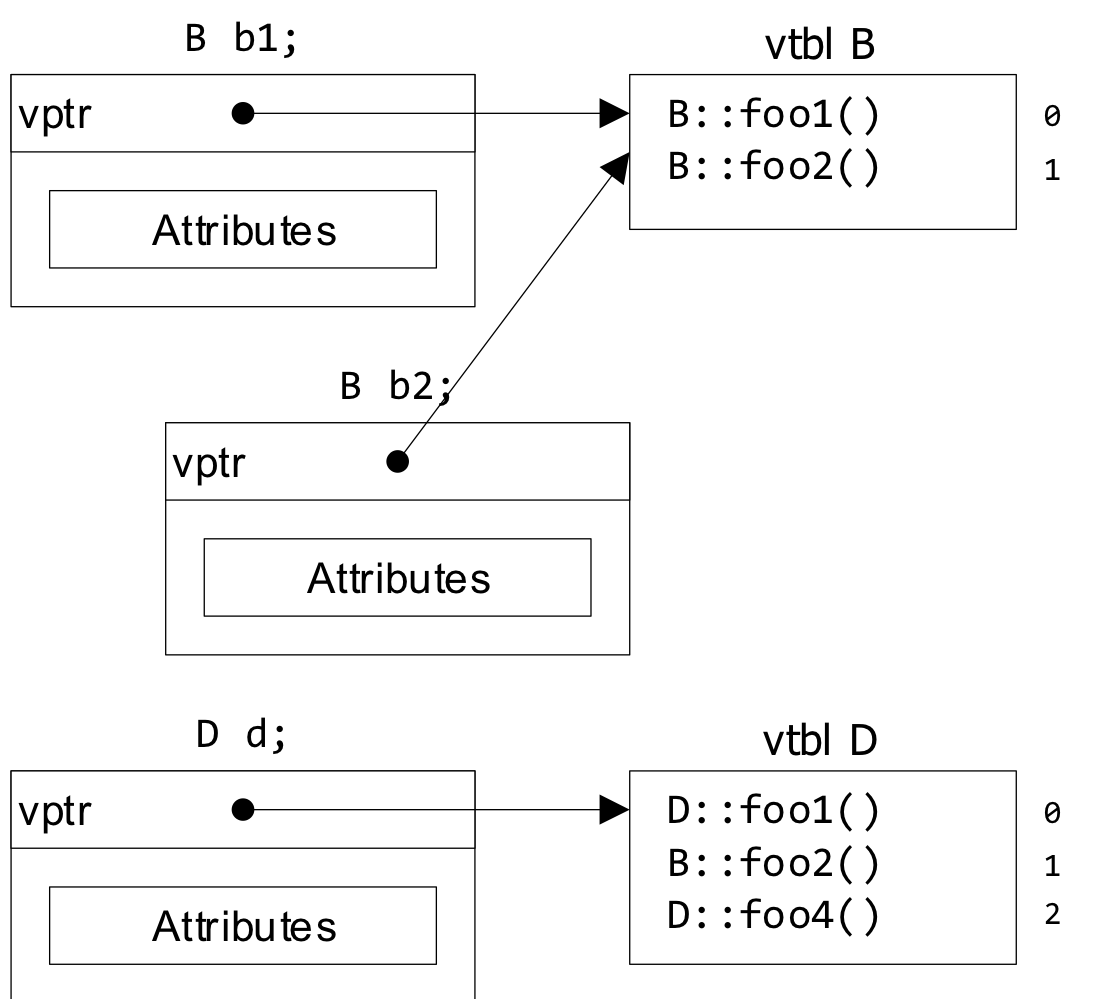
\includegraphics[width=\linewidth]{images/vtable.png}
\end{minipage}



\subsection{Abstrakte Klassen}

Wenn Klassen zwar festlegt, dass eine Methode da ist, diese aber noch nicht implementieren, nennt man das eine abstrakte Methode. 
Man spricht dann von einer abstrakten Klasse.
Eine abstrakte Methode wird in UML \textit{\textbf{kursiv}} dargestellt.
Es ist egal, ob die abstrakten Methoden selbst definiert sind oder geerbt. 
Abstrakte Klassen kann man nicht instanziieren.
Es gibt kein spezielles Schlüsselwort dafür, man weist der Methode bei Definition 0 zu: 

\lstinputlisting{code/03_Objektorientierung/abstraktemethode.cpp}

\subsection{Organisation der H files}

Generell gilt immer noch: Jedes H File hat ein Cpp File. 
Allerdings können Unterklassen in ein H File zusammengefasst werden, falls diese nicht allzu Umfänglich sind. 
Ansonsten sollte ein neues H File erstellt werden. 
Für abstrakte Klassen fällt die Implementierung in einem Cpp file weg.

\subsection{Mehrfachvererbung}

Folgender Vererbungszweig ist möglich:\\
\noindent
\begin{minipage}{0.38\columnwidth}
        \begin{tikzpicture}[
    node distance=0.4cm and 0.2cm,
]

    % Nodi
    \node[umlclass] (c1) {\textbf{C1}\nodepart{second}\nodepart{third}};
    
    \node[umlclass, below left=of c1] (c2) {\textbf{C2}\nodepart{second}print()\nodepart{third}};
    \node[umlclass, below right=of c1] (c3) {\textbf{C3}\nodepart{second}print()\nodepart{third}};
    
    % C4 posizionato centralmente sotto C2 e C3
    \node[umlclass, below=2cm of c1] (c4) {\textbf{C4}\nodepart{second}\nodepart{third}};

    % Connessioni
    \draw[inheritance] (c2) -- (c1);
    \draw[inheritance] (c3) -- (c1);
    \draw[inheritance] (c4) -- (c2);
    \draw[inheritance] (c4) -- (c3);

\end{tikzpicture} 
\end{minipage}
\begin{minipage}{0.62\columnwidth}
Solche Gebilde sind zwar möglich, sollten jedoch vermieden werden, da schnell sehr kompliziert und kaum lesbar. 
Es entsteht schnell Mehrdeutigkeit durch die verschiedenen Erbzweige.\\

Se nelle 2 classi parenti è definito un \cor{\textbf{metodo} con lo \textbf{stesso nome}}, è necessario
ridefinitrlo nella sottoclasse definendo il giusto comportamento (ad es. \lstinline[language=C++]|C1::print()|)
\end{minipage}

Bei der Definition einer Klasse können weitere Oberklassen mit einem Komma getrennt angegeben werden
\lstinputlisting{code/03_Objektorientierung/Mehrfachvererbung.cpp}\vspace{-1em}

\subsubsection{Diamond Problem}

\begin{itemize}
    \item \textbf{Il Problema}: Senza accorgimenti, \texttt{C4} conterrebbe due copie 
    separate di \texttt{C1} (tramite \texttt{C2} e tramite \texttt{C3}). 
    \cor{Generando ambiguità nell'accesso ai membri.}
    \item \textbf{La Soluzione (\textit{Virtual Inheritance})}:la parola 
    chiave \texttt{virtual} nelle classi intermedie (\texttt{C2} e \texttt{C3})
    istruisce il compilatore a creare un'unica istanza condivisa di \texttt{C1}.
    \item \textbf{Ordine di Inizializzazione}: Segue una priorità gerarchica:
    \begin{enumerate}
        \item \textbf{Base Virtuale}: \texttt{C1} viene inizializzata per prima.
        \item \textbf{Basi Non-Virtuali}: \texttt{C2} e poi \texttt{C3} (seguendo l'ordine di dichiarazione in \texttt{C4}).
        \item \textbf{Classe Derivata}: Il corpo del costruttore di \texttt{C4}.
    \end{enumerate}
\end{itemize}

\lstinputlisting[language=C++]{code/03_Objektorientierung/03_Objektorientierung_snippet_3.cpp}
\subsection{Static} 

Static im Zusammenhang mit Klassen bindet eine Methode oder ein Attribut an die Objektklasse und nicht an die Objektinstanz (ähnlich zu Python Klassenvariablen).


\subsubsection{Methoden}

Static Methoden müssen im Header-File deklariert und im Cpp-File definiert werden. 
Sie dürfen nur auf Static definierte Attribute zugreifen da \textbf{keine Objektinstanz vorhanden.} 
Hauptanwendungen sind Hilfsfunktionen wie Funktionsaufrufcounter oder Umrechnungsfunktionen. 
Bei der Deklaration wird der Klassennamen verwendet (siehe Bsp). 

\subsubsection{Attribute}

Static Attribute müssen im H deklariert \textbf{und im Cpp File} definiert werden. 
Sie werden verwendet für z.B. Objektspezifische Konstanten oder im Zusammenhang mit Static Counter. 
(\textit{class scope})

\subsubsection{Bsp}

\lstinputlisting{code/03_Objektorientierung/static.cpp}